\documentclass[hidelinks,12pt]{article}
\usepackage[english,brazil]{babel}
\usepackage{hyperref}
\usepackage{graphicx}
\graphicspath{ {images/} }
\linespread{1.3}

\usepackage{geometry}
\geometry{
	a4paper,
	top=30mm,
	left=30mm,
	right=20mm,
	bottom=20mm
}

\usepackage{float}
\usepackage{subcaption}

\usepackage{listings}

\usepackage[titletoc,title]{appendix}
\usepackage{bookmark}
\makeatletter
\renewcommand*\l@section{\@dottedtocline{1}{0em}{1.5em}}
\makeatother
\author{Bruno Yoshikazu Shimada}
\title{\textbf{Desenvolvimento de aplicativo Android paara Micropagamentos}
	}
\date{Novembro 2017}

\begin{document}
\begin{titlepage}
	\centering
	{\Large Universidade de S\~ao Paulo\par}
	{\Large Escola de Artes, Ci\^encias e Humanidades\par}
	\vfill
	{\Large Bruno Yoshikazu Shimada\par}
	\vspace{1cm}
	{\Large\bfseries Desenvolvimento de aplicativo para micropagamentos na plataforma Android\par}
	\vfill
	{\Large S\~ao Paulo\par}
	{\Large 2017\par}
\end{titlepage}
\newpage
\begin{titlepage}
	\centering
	{\Large Bruno Yoshikazu Shimada\par}
	\vspace{2cm}
	{\Large\bfseries Desenvolvimento de aplicativo para micropagamentos na plataforma Android\par}
	\vfill
	\begin{flushright}
		\hspace{7cm}Relat\'orio parcial apresentado \`a Escola de Artes,
	
		\hspace{7cm}Ci\^encias e Humanidades, da Universidade de S\~ao
	
		\hspace{7cm}Paulo, como parte dos requisitos exigidos na
	
		\hspace{7cm}disciplina ACH 2018 - Projeto Supervisionado ou
	
		\hspace{7cm}de Gradua\c{c}\~ao II, para obten\c{c}\~ao do t\'itulo de
	
		\hspace{7cm}Bacharel em Sistemas de Informa\c{c}\~ao.
		\bfseries Orientador: Prof. Dr. Luciano Vieira de Ara\'ujo
		
		Modalidade: TCC curto (1 semestre) - individual
	\end{flushright}
	\vspace{2cm}
	{\Large S\~ao Paulo\par}
	{\Large 2017\par}
\end{titlepage}
\newpage
\begin{titlepage}
	\begin{flushleft}
		{\Large Nome: SHIMADA, Bruno Yoshikazu \par}
		{\Large T\'itulo: Desenvolvimento de aplicativo para micropagamentos na plataforma Android \par}
	\end{flushleft}
	\begin{flushright}
		\hspace{7cm}Relat\'orio parcial apresentado \`a Escola de Artes,
		
		\hspace{7cm}Ci\^encias e Humanidades, da Universidade de S\~ao
		
		\hspace{7cm}Paulo, como parte dos requisitos exigidos na
		
		\hspace{7cm}disciplina ACH 2018 - Projeto Supervisionado ou
		
		\hspace{7cm}de Gradua\c{c}\~ao II, para obten\c{c}\~ao do t\'itulo de
		
		\hspace{7cm}Bacharel em Sistemas de Informa\c{c}\~ao.
	\end{flushright}
	\vspace{1cm}
	\begin{flushleft}
		{\Large Aprovado em: \rule{1cm}{1pt}/\rule{1cm}{1pt}/\rule{2cm}{1pt} \par}
	\end{flushleft}
	\vfill
	\centering
		{\Large Banca Examinadora \par}
		\vspace{1cm}
		\begin{flushleft}
			{\Large Prof. Dr:\rule{5cm}{1pt}    Institui\c{c}\~ao:\rule{5cm}{1pt}\par}
			{\Large Julgamento:\rule{4,2cm}{1pt} Assinatura:\rule{5cm}{1pt}\par}
			\vspace{1cm}
			{\Large Prof. Dr:\rule{5cm}{1pt}    Institui\c{c}\~ao:\rule{5cm}{1pt}\par}
			{\Large Julgamento:\rule{4,2cm}{1pt} Assinatura:\rule{5cm}{1pt}\par}
			\vspace{1cm}
			{\Large Prof. Dr:\rule{5cm}{1pt}    Institui\c{c}\~ao:\rule{5cm}{1pt}\par}
			{\Large Julgamento:\rule{4,2cm}{1pt} Assinatura:\rule{5cm}{1pt}\par}
		\end{flushleft}
\end{titlepage}
\newpage
\selectlanguage{brazil}
\section*{\centering{Agradecimentos}}
\pagenumbering{roman}
Agrade\c{c}o \`a todos que me incentivaram, deram suporte e n\~ao me deixaram desistir ao longo do caminho trilhado na faculdade. Agrade\c{c}o aos meus pais pelo apoio e incentivo de buscar entrar na USP, agrade\c{c}o aos colegas que me ajudaram em momentos de dificuldade, agrade\c{c}o aos amigos que nunca me abandoram e sempre estiveram ao meu lado, agrade\c{c}o a toda comunidade da EACH que me ajudaram a crescer como ind\'ividuo permitindo ver que a vida \'e muito mais do que imaginamos e conhecemos. Agrade\c{c}o ao corpo docente da EACH, tanto da \'area de Sistemas de Informa\c{c}\~ao como os de outras \'areas conhecids durante o Ciclo B\'asico. Agrade\c{c}o ao Prof. Dr. Luciano Vieira de Araújo por me orientar neste trabalho, agrade\c{c}o ao Henrique Leme, desenvolvedor principal da plataforma de servi\c{c}os usada, pelo apoio durante o desenvolvimento das interfaces e integra\c{c}\~oes.
\newpage
\selectlanguage{brazil}
\section*{\centering{Gloss\'ario}}


\hspace{0.5cm}\textbf{Android}: Sistema operacional \textit{open source} baseado em \textit{Linux} desenvolvido pela \textit{Google} para uso em \textit{smartphones} e \textit{tablets}.
\newline

\textbf{\textit{UI}}: \textit{User Interface} é a interface entre o usuário e o sistema na qual o usuário tem controle sobre as ações executadas.
\newline

\textbf{\textit{Material Design}}: Uma linguagem de design desenvolvida pela \textit{Google} que visa servir como guia para o desenvolvimento de interfaces.
\newline

\textbf{\textit{Java}}: Linguagem de programação desenvolvida sob licença \textit{GNU} e desenvolvida pela \textit{Sun Microsystems}, e mantida pela \textit{Oracle}
\newline

\textbf{\textit{XML}}: Linguagem de marcação composto por uma sequência de pares atributo e valor, de fácil interpretação pela máquina e por humanos.
\newpage
\selectlanguage{brazil}
\section*{\centering{Resumo}}

Vivemos em uma \'epoca que a cada dia, novas solu\c{c}\~oes digitais s\~ao lan\c{c}adas para resolver nossos problemas cotidianos de uma maneira simplificada que se incorporam ao nosso cotidiano de uma maneira que ap\'os algum tempo n\~ao conseguimos imaginar como n\'os conseguimos viver sem isso por tanto tempo.

Entre as solu\c{c}\~oes digitais podemos citar por exemplo o ramo econ\^omico e banc\'ario, com desde os b\'asicos aplicativos de bancos para consulta a extratos, pagamentos de boletos, etc, at\'e solu'\c{c}\~oes mais sofisticadas como aplicativos para receber e processar pagamentos por cart\~ao.

Por\'em um problema corriqueiro que temos no dia-a-dia \'e o pagamento de pequenas transa\c{c}\~oes monet\'arias, como tomar um caf\'e na padaria, comprar um chiclete na bomboniere, emprestar uma pequena quantia de dinheiro para um conhecido, entre outras que na maioria das vezes n\~ao passam de 10R\$ e que geram uma perda de tempo de ter que realizar o pagamento com um cart\~ao, digitando a senha pessoal em uma m\'aquina e torcendo para o servi\c{c}o da operadora do cart\~ao estar disponível no momento.

Para resolver esse problema entram em cena os servi\c{c}os de micropagamento, que buscam solucionar o problema de fazer um pagamento ou uma transa\c{c}\~ao de pequeno valor entre duas pessoas, independente de ser pessoa-a-pessoa ou pessoa-a-neg\'ocio, de forma r\'apida, eficaz, segura e descomplicada. O prop\'osito deste trabalho \'e ent\~ao desenvolver um aplicativo Android, SO mais comum entre os usu\'arios de celular no Brasil, que gerencie as transações entre usu\'arios do aplicativo e que fa\c{c}a valer as caracter\'isticas descritas anteriormente.
\newline



\textbf{Palavras Chaves}
\begin{itemize}
	\item Micropagamentos
	\item \textit{Android}
	\item \textit{Fintech}
\end{itemize}
\newpage
\selectlanguage{english}
\begin{abstract}
We live in time that everyday new digital solutions are released to solve our daily problems in a simplified manner, that merges into our days that after some time we are unable to imagine how we lived so much time without it.

Among these digital solutions we can mention for example the economic/banking areas, that has the basic bank app for checking account information, payment of tickets, etc.. To more sophisticated apps that receive and process payments by card.

However a common problem we have in our daily lives is the payment of small monetary transactions, such as having a coffee at a bakery, buying gum from a local store, lending money to an acquaintance, among others that in most times don’t surpass 10 BRL and generate a loss of time for having to make the payment with a card, typing our personal password on a machine and hoping the service of the card operator will be available at the moment.

To solve this problem the micropayments services come into play, seeking to solve the problem of making the payment or transaction of a small amount of money between two persons, regardless of being a person-to-person or person-to-business, in a quick, efficient, safe and uncomplicated way. The purpose of this work is to develop an Android app, the most common OS among mobile users in Brazil, that manage transaction between users of the app and enforce the characteristic described before.
\newline


\textbf{Keywords}
\begin{itemize}
	\item Micropayments
	\item Android
	\item Fintech
\end{itemize}
\end{abstract}
\newpage
\selectlanguage{brazil}
\begingroup
\centering
\listoffigures
\endgroup
\newpage
\selectlanguage{brazil}
\begingroup
\hypersetup{hidelinks}
\tableofcontents
\endgroup
\newpage
\pagenumbering{arabic}
\selectlanguage{brazil}
\section{Introdu\c{c}\~ao}
A defini\c{c}\~ao de micropagamento \'e relativamente simples, se usado uma associa\c{c}\~ao das palavras que a comp\~oem, se infere que se trata de transa\c{c}\~oes cujo valor \'e uma quantia muito pequena. Trazendo para a realidade dele, um micropagamento \'e uma transa\c{c}\~ao online de uma quantia muito pequena de dinheiro (INVESTOPEDIA). Qu\~ao pequeno esse valor \'e, varia entre as diferentes empresas no mercado, o \textit{PayPal}, \textit{e-commerce} que faz a transa\c{c}\~ao de valores digitais entre usu\'arios nas duas pontas, considera um micropagamento qualquer transa\c{c}\~ao cujo valor seja menor do que 10USD (PAYPAL).

A evolu\c{c}\~ao do mercado de  micropagamentos \'e creditada a 3 fatores \textit{(HERNANDEZ - VERME,BENAVIDES;2013)} definidos com base em um relat\'orio de \textit{VASILJEV(2016)} e \textit{BURELLI (2016)}, definem eles como: 
\begin{itemize}
	\item O crescimento da infraestrutura de rede e do e-commerce em geral
	\item O crescimento das redes sociais, jogos online e neg\'ocios de bens digitais
	\item O aparecimento de novas formas de servi\c{c}os de pagamento online
\end{itemize}
Com base nisso podemos ver que as solu\c{c}\~oes atuais para micropagamento surgiram principalmente da necessidade de pagamento de bens para consumo digital como assinaturas de sites, compras de m\'usicas digitais, o melhor exemplo aqui seria o \textit{iTunes} por exemplo.
Dentre as solu\c{c}\~oes que existem atualmente, a \textit{Investopedia} d\'a foco em dois modelos:
\begin{itemize}
	\item A plataforma agindo como carteira digital. Cada usu\'ario cria sua conta na plataforma que ir\'a gerenciar a transa\c{c}\~ao entre dois usu\'arios, a transa\c{c}\~ao \'e efetuada e a plataforma se encarrega de armazenar esse valor, quando a carteira de qualquer uma dessas partes atinge um limite, a quantia total do dinheiro e liberada e transferida para o usu\'ario.
	\item A plataforma agindo com cr\'editos. Cada usu\'ario cria sua conta no plataforma, cada um deles compra/recarrega a quantia desejada que deseja ter como cr\'edito, a cada transa\c{c}\~ao entre duas partes a plataforma se encarrega de atualizar os cr\'editos de ambas as partes.
\end{itemize}
O grande problema na \'area de micropagamentos s\~ao as taxas cobradas pelas operadoras de cart\~ao de cr\'edito, meio que a maioria dos modelos existentes como demonstrado acima usa como forma preferencial de pagamento o cart\~ao cr\'edito, por\'em \'e sabido que para cada transa\c{c}\~ao s\~ao cobradas taxas em cima do valor pago, \'e um caso raro mas podem existir situa\c{c}\~oes que as taxas podem, porque n\~ao, superar o valor da transa\c{c}\~ao, o que para um cliente que seja dono de um neg\'ocio, torna-se algo insustent\'avel.

Uma plataforma de micropagamentos tamb\'em pode se aplicar ao mundo offline como uma forma de currência que substitua o dinheiro padr\~ao em pequenas comunidades.

Imagine por exemplo o ambiente de um condom\'inio privado que ofer\c{c}a servi\c{c}os internos para os condôminos, a forma natural que se imagina que as transa\c{c}\~oes v\~ao ocorrer nesse meio \'e por forma de dinheiro em esp\'ecie, o que levanta alguns riscos para essa popula\c{c}\~ao, sabendo que nessa ambiente circula dinheiro vivo, e que a seguran\c{c}a \'e alguns n\'iveis mais baixa que a comum, alguma pessoa mal intencionada pode pensar em levar vantagem e cometer um assalto contra os prestadores desse servi\c{c}o visando roubar o dinheiro que fica acumulado.

Com o uso de uma plataforma de micropagamentos os condôminos poderiam fazer a carga de uma quantia de dinheiro digital em um aplicativo, os prestadores de servi\c{c}o aceitarem essa forma de pagamento, e a pessoa fazer a transa\c{c}\~ao usando esse dinheiro digital, isso faz com que n\~ao circule dinheiro vivo no ambiente deles, o dinheiro est\'a circulando, por\'em ele est\'a externo ao ambiente, ele n\~ao pode ser acessado de uma maneira f\'isica naquele local o que pode ajudar a inibir pessoas que pensem em roubar o condom\'inio j\'a que n\~ao haveria dinheiro f\'isico no local.

Essa mesma abordagem pode ser aplicada para por exemplo, o restaurante universit\'ario da nossa faculdade. Ao inveś de pagar a carga do cart\~ao com o dinheiro f\'isico, os alunos poderiam fazer isso com um aplicativo, efetuando a carga de cr\'editos com um cart\~ao de cr\'edito por exemplo e pagando na entrada com o seu celular e a funcion\'aria do restaurante com o celular da empresa respons\'avel recebendo os pagamentos.
\newpage
\section{Objetivos}


\subsection{Objetivo Geral}
O objetivo do trabalho foi desenvolver um aplicativo \textit{Android} que conseguisse efetuar micropagamentos entre \textit{smarthphones}.
\newline


\subsection{Objetivos Espec\'ificos}
Os objetivos espec\'ificos do trabalho foram:
\begin{itemize}
	\item Aprendizagem do conceito de micropagamentos
	\item Estudo da bibliografia de artigos de micropagamentos.
	\item Desenvolver a \textit{UI} do aplicativo 
	\item Integrar a interface com base em uma plataforma de servi\c{c}os e infraestrutura existente.
\end{itemize}
\newpage
\section{Revis\~ao Bibliogr\'afica} \label{revisao}
Ao longo do desenvolvimento do aplicativo, em diversos momentos apareceram d\'uvidas que n\~ao conseguiam ser resolvidas por for\c{c}a bruta, como por exemplo, como definir a posi\c{c}\~ao fixa de um bot\~ao em rela\c{c}\~ao a outros no mesmo layout? D\'uvidas desde as mais simples, que surgem principalmente nos momentos iniciais de aprendizado de alguma linguagem ou \textit{framework} novo, at\'e as mais complexas, quando j\'a se tem uma base s\'olida de conhecimento sobre o t\'opico, s\~ao comuns no meio da tecnologia, fato que pode ser comprovado fazendo uma simples busca no \textit{Google}, nas p\'aginas de resultado \'e comum encontrar pessoas com a mesma d\'uvida, em variados f\'oruns, blogs e  sites diversos. O mais interessante nesse ponto \'e a tamb\'em a variedade de abordagens diferentes que s\~ao poss\'iveis de encontrar para uma mesma d\'uvida, fazendo com que tenhamos que filtrar dentre elas a que melhor se aplica ao contexto do nosso problema.

Abaixo est\~ao listadas as fontes consultadas ao longo do trabalho que ajudaram em diversos momentos do desenvolvimento.

Para entendimento do conceito de micropagamentos foram usadas duas fontes principais.

A p\'agina do termo \cite{invest} no site da \textit{Investopedia} que deu uma vis\~ao geral sobre o assunto, enfocando primeiro em um resumo simplificado para depois se aprofundar um pouco mais nele. O interessante desse site \'e que a partir do termo \textit{"micropayment"}, ele busca termos relacionados buscando fazer uma trilha de informa\c{c}\~oes para abranger o assunto.

Outra fonte consultada foi o artigo \textbf{\textit{"Virtual currencies, micropaymentes and the payments systems: a challenge to fiat money and monetary policy?"}} \cite{microp} que discorre n\~ao s\'o sobre o conceito de micropagamentos como tamb\'em aborda o tema das moedas virtuais e relaciona ambos. O artigo foca mais na parte de como os micropagamentos s\~ao mais relevantes no mundo online na compra de itens que eles classificam como microprodutos, fazem uma compara\c{c}\~ao das transa\c{c}\~oes online que envolvem produtos f\'isicos e digitais. Esse artigo considero como o principal usado j\'a que ele aborda de uma maneira mais aprofundada o ambiente que os micropagamentos se inserem.

O artigo \textbf{\textit{"Micropayments: A Viable Business Model?"}} \cite{stanford} apresenta um ponto interessante nas quest\~oes sobre os desafios t\'ecnicos que uma aplica\c{c}\~ao de micropagamentos teria que se preocupar em atender para desenvolver uma aplica\c{c}\~ao segura. Os autores listam 5 pontos que consideram serem desafios que precisam ser vencidos para uma implementa\c{c}\~ao bem-sucedida, seguran\c{c}a, escalabilidade, confiabilidade, interoperabilidade e anonimidade. O interessante desse artigo \'e ele fazer o relacionamento do ecossistema de micropagamentos com os componentes e requisitos desej\'aveis para desenvolvimento de um aplicativo. 

Seguran\c{c}a \'e um requisito necess\'ario para praticamente qualquer aplicativo, por\'em quando tal aplica\c{c}\~ao envolve dinheiro e transa\c{c}\~oes ele se torna um problema de alta prioridade de ser resolvido, ter um aplicativo inseguro que apresente muitas falhas, e entre elas as que sujeitam o aplicativo a sofrer ataques que comprometam as informa\c{c}\~oes e dados de usu\'arios, podem fazer a confian\c{c}a nele cair, o que reduz a base de usu\'arios. Os autores nesse item que durante o desenvolvimento \'e preciso tomar aten\c{c}\~ao com autentica\c{c}\~ao, autoriza\c{c}\~ao, integridade de informa\c{c}\~ao e confidencialidade.

Arquitetar o sitema de uma maneira que permita que ela seja escal\'avel \'e um requisito necess\'ario para poder lidar com um pontencial aumento do n\'umero de acessos a aplica\c{c}\~ao. O desenho da solu\c{c}\~ao deve ser de tal forma que seja poss\'ivel acoplar mais servidores a medida que foram necess\'arios para poder lidar com o tr\'afego de informa\c{c}\~oes.

\'E levantado tamb\'em a quest\~ao de interoperabilidade, permitir que diferentes aplica\c{c}\~oes de micropagamentos conversem entre si, este talvez seja o ponto de maior dificuldade de se atingir. Aplica\c{c}\~oes diferentes possuem diferentes meios de tratar a informa\c{c}\~ao que chega, sai, e processada nele.


A quest\~ao da anonimidade \'e tratado como um ponto complicado de se definir, at\'e que ponto a anonimidade deve existir a a partir de que ponto \'e necess\'ario saber a identididade dos usu\'arios, quanto um usu\'ario pode e deve saber do outro, quest\~oes que valem para os dois atores envolvidos em um micropagamento. O artigo n\~ao levanta nennhuma resposta definitiva sobre o assunto, ele apresenta bons argumentos a favor e contra a quantidade de anonimidade no sistema.

Um dos exemplos \'e explorado \'e o registro de hist\'orico de transa\c{c}\~oes, para um usu\'ario que faz o pagamento \'e uma informa\c{c}\~ao \'util de ser acessada, mas que precisa de uma pequena fra\c{c}\~ao de depriva\c{c}\~ao de anonimidade. Mas ao mesmo tempo \'e informa\c{c}\~ao que pode ser usada por terceiros para descobrir padr\~oes de consumo e o que foi consumido, e que pode ser usado contra o usu\'ario. Um \textit{e-commerce} por exemplo, com base nessas informa\c{c}\~oes pode manipular os pre\c{c}os e an\'uncios que tem potencial de ser interesse de tal usu\'ario.
% link do training para android

No come\c{c}o do projeto meu conhecimento de programa\c{c}\~ao para \textit{Android} era nulo, durante a prepara\c{c}\~ao da m\'aquina encontrei no mesmo site que disponibiliza a \textit{IDE} para desenvolvimento, uma sub-se\c{c}\~ao intitulada \textit{Training}, debaixo da se\c{c}\~ao \textit{Develop} \cite{anddev}. Nela encontrei uma s\'erie de li\c{c}\~oes b\'asicas para quem est\'a come\c{c}ando a desenvolver para \textit{Android}. Foi \'util para ter uma no\c{c}\~ao b\'asica de onde come\c{c}ar e os termos espec\'ificos usados.

Ap\'os a cria\c{c}\~ao de um aplicativo \textit{Hello World} b\'asico seguindo o guia \cite{androidhw} do site da \textit{Android}, fui atr\'as de mais algum material para criar um aplicativo e aprofundar um pouco mais o conhecimento na plataforma. O livro \cite{andppe} utilizado nesse momento foi \textbf{\textit{"Android 5 Programming by Example"}}, o livro \cite{andppe} se aprofunda um pouco mais nos exerc\'icios ajudando e servindo de guia para criar um aplicativo mais robusto do que o visto no guia do site da \textit{Android}. O livro \cite{andppe} foi usado de guia no segundo passo do projeto onde criei um aplicativo \textit{mock} que simulava localmente uma transa\c{c}\~ao nos moldes de um micropagamento de um aparelho para um servidor, para testar os conhecimentos e novas t\'ecnincas adquiridas. Apesar do livro \cite{andppe} focar mais na vers\~ao \textit{Lollipop}, lan\c{c}ada em 2015 mesmo ano da publica\c{c}\~ao do livro, grande parte dos componentes n\~ao mudou muito para a vers\~ao mais atual.


Durante a elabora\c{c}\~ao do rascunho das interfaces do aplicativo uma p\'agina \cite{material} que foi muita usada como fonte de consulta e guia \'e a \textit{Material Design}. Nela foi poss\'ivel encontrar orienta\c{c}\~oes e guias de como desenhar a interface para se encaixar no padr\~ao do \textit{Material Design}. A seguir s\~ao descritas as ferramentas e guias dispon\'iveis que se destacam pelo seu uso e importância no projeto.

A p\'agina \textbf{\textit{Material Icons}} \cite{materialicon} \'e uma esp\'ecie de repos\'itorio da \textit{Google} com v\'arios \'icones dispon\'iveis para uso. Todos s\~ao liberados para uso sobre a licen\c{c}a \textit{Apache License Version 2.0}. Os \'icones s\~ao desenhados de maneira simples e de f\'acil interpreta\c{c}\~ao, o design deles \'e de uma maneira que quando se olha para o \'icone \'e f\'acil deduzir qual seu significado. Por exemplo o \'icone da figura \ref{icon_pay} que foi usado para simbolizar a a\c{c}\~ao de pagamento:
	% (inserir \'icone do pagamento)
	\begin{figure}[h]
		\centering
		
\includegraphics{pay_action_white}
		\caption{\'Icone usado para simbolizar a a\c{c}\~ao de pagamento}
		\label{icon_pay}
	\end{figure}

	Al\'em da p\'agina com o rep\'ositorio dos \'icones, o design e o conceito dos itens \'e explicado no artigo \textbf{\textit{Style - Icons}} \cite{materialiconguide}
	
A p\'agina \textbf{\textit{Material Colors}} \cite{materialcolors} possui uma ferramenta \cite{materialcolorpallete} que ajuda na escolha da paleta de cores que v\~ao compor o aplicativo, ele oferece tamb\'em um guia visual de como ficam as cores nas interfaces do sistema. Outro artigo relacionado \'e \textbf{\textit{Style - Colors}} \cite{materialcolors} onde \'e explicado as boas pr\'aticas e guias para selecionar as cores dos componentes da interface do aplicativo.

\newpage
\section{Metodologia}

Para o projeto eram necess\'arios conhecimentos em dois t\'opicos, micropagamentos e \textit{Android}. Inicialmente foi feito um estudo da bibliografia de micropagamentos, descrita no cap\'itulo \ref{revisao}, para entender melhor o conceito dele como um todo, suas caracter\'isticas, limites, o panorama atual e o mercado. Tendo aprendido esse conceito foi feito um estudo buscando aprender os conceitos da programa\c{c}\~ao para \textit{Android}, posteriormente foram desenvolvidos alguns aplicativos de teste para aplicar o conhecimento adquirido.

Adquiridos os fundamentos necess\'arios sobre os dois assuntos dei andamento no trabalho para definir o escopo dele, foram definidas quantas e quais interfaces seriam necess\'arias para atingir o objetivo proposto, desenvolver a interface de um aplicativo \textit{Android} com base numa plataforma de servi\c{c}os existentes buscando fazer a mesma ser simples, no sentido de ter uma f\'acil utiliza\c{c}\~ao, buscando obedecer e seguir os guias definidos pelo \textit{Android} como boas pr\'aticas e que atendem e se adequam a filosofia do \textit{Material Design}. Foram avaliados nesse momento as estruturas e componentes que seriam usados, como por exemplo bot\~oes, layouts, esquema de cores, etc.

Definida as interfaces passei a avaliar a estrutura de servi\c{c}os com as quais as interfaces seriam integradas, foi o momento de aprender como funcionava a plataforma, como ela se comunicava internamente entre suas classes, quais eram as entradas e sa\'idas de cada momento. Com isso foi refinado a etapa anterior de defini\c{c}\~ao das interfaces para se adequar a plataforma, foram revistas as interfaces imaginadas,adicionando e retirando alguns componentes visuais, e criadas novas interfaces.

Com o escopo definido foi feito uma avalia\c{c}\~ao de esfor\c{c}o para definir o cronograma que seria seguido e dado in\'icio ao desenvolvimento das interfaces do aplicativo.

Para o desenvolvimento das interfaces do aplicativo, e controle das a\c{c}\~oes foram utilizadas duas linguagens no trabalho:
\begin{itemize}
	\item \textbf{\textit{XML}}: todas as interfaces do \textit{Android} s\~ao escritas usando a linguagem de marca\c{c}\~ao \textit{XML}, o \textit{Android} usa um conjunto de elementos e atributos pr\'oprios na marca\c{c}\~ao como por exemplo o elemento \textit{\textless{RelativeLayout}\textgreater} e o atributo \textit{android:layout\_width}. \textit{XML} tamb\'em usado para definir \textit{Strings}, o tema base, e qualquer outro elemento visual que possa ser reaproveitado, como por exemplo um \textit{layout} customizado para um bot\~ao. Tamb\'em \'e usado para definir o manifesto do aplicativo, onde s\~ao declaradas configur\~a\c{c}\~oes espec\'ificas do aplicativo, como por exemplo permiss\~ao para uso de \textit{bluetooth}, \textit{internet}, etc.
	\item \textbf{\textit{Java}}: A parte do \textit{back-end} que controla a aplica\c{c}\~ao \'e toda codificada em \textit{Java}. O \textit{Android} usa \textit{Java} para por exemplo codificar um \textit{listener} que capta quando o usu\'ario clica em algum bot\~ao por exemplo, para fazer a troca de interfaces, controle de sess\~ao, carregar \textit{Strings} dinâmicas na interface, tratamento de erros e exce\c{c}\~oes, etc.
\end{itemize}

Quanto a \textit{hardware} foram usados um \textit{notebook} pr\'oprio rodando um SO \textit{Debian}, e dois aparelhos celulares pr\'oprios com SO \textit{Android} para simular o comportamento de dois usu\'arios. Devido a diferen\c{c}a de SO de ambos, foi interessante observar como a interface se comportava em cada um deles. A t\'itulo de curiosidade seguem as especifica\c{c}\~oes:
\begin{itemize}
	\item \textit{Notebook}
	\begin{itemize}
		\item SO: \textit{Ubuntu 16.04 LTS - 64-bit}
		\item Mem\'oria RAM: 8GB
		\item Processador: \textit{Intel\textregistered Core\textsuperscript{TM} i7-5500U CPU @ 2.40GHz x 4}
		\item Processador gr\'afico: \textit{Intel\textregistered HD Graphics 5500 (Broadwell GT2)}
	\end{itemize}
	\item Celular \textit{Motorola Moto G} 3\textsuperscript{\underline{a}} Gera\c{c}\~ao
	\begin{itemize}
		\item SO: \textit{Android 5.1 Lollipop}
		\item Mem\'oria RAM: 1GB
		\item Processador: \textit{Qualcomm Snapdragon 410}
	\end{itemize}
	\item Celular \textit{Samsung S3 Mini}
	\begin{itemize}
		\item SO: \textit{Android 4.1 Jellybean}
		\item Mem\'oria RAM: 1GB
		\item Processador: \textit{Dual-core, 1000 MHz}
	\end{itemize}
\end{itemize}
\newpage
\section{Resultados}

\subsection{Desenvolvimento das interfaces} \label{learn}
% start new block
Foram definidas inicialmente para o trabalho o desenho de 4 interfaces, \textit{login}, uma tela principal com as a\c{c}\~oes permitidas ao usu\'ario, a tela de efetuar o micropagamento e a tela de confirma\c{c}\~ao do pagamento, ap\'os estudo da estrutra da plataforma de servi\c{c}os e revis\~ao das interfaces, o n\'umero de interfaces que seriam necess\'arias ficou em 13. Para cada uma delas ser\'a descrita o que foi feito e os componentes usados.

Para o desenvolvimento das interfaces foi levantado duas abordagens diferentes, o uso de \textit{RelativeLayout} ou o uso do \textit{ConstraintLayout}, ambas alternativas foram testadas para mensurar as possibilidades e dificuldades que cada uma apresentava, por fim foi escolhido seguir o desenvolvimento usando o primeiro. A vantagem no uso do \textit{Relative Layout} \'e poder declarar a posi\c{c}\~ao dos componentes de acordo com seus parentes ou seus irm\~aos, ele d\'a um maior controle sobre os itens no \textit{layout}. Por exemplo, temos uma \textit{view} que define uma \'area retangular na interface, e dentro dessa \'area precisam estar 3 outros componentes, vamos dizer bot\~oes, e esses 3 componentes precisam estar alinhados à direita da \'area. Com o \textit{RelativeLayout} declaramos a \'area, o primeiro bot\~ao alinhado a direita da \'area, e cada um dos bot\~oes subsequentes um abaixo do outro, com a \textit{ConstraintLayout} o mesmo processo precisa que algumas propriedades a mais sejam usadas para obter o mesmo resultado.

A primeira interface a ser feita foi a de cadastro de us\'ario (imagem \ref{cadastro}). No fluxo de execu\c{c}\~ao normal, essa interface \'e a primeira, por\'em ela deve ocorrer apenas uma vez no momento que o usu\'ario vai se cadastrar, se o usu\'ario j\'a fez o cadastro essa tela n\~ao volta a ser exibida sendo exibida no seu lugar a interface de \textit{login} (imagem \ref{login}).

Para a interface de cadastro (imagem \ref{cadastro}) foram necess\'arios avaliar e estudar a implementa\c{c}\~ao de três tipos de componentes: \textit{EditText}, \textit{Button} e \textit{ImageView}, os três componentes n\~ao apresentaram grande dificuldade em assimilar o comportamento e o que deveria ser feito para aplicar na interface.
\begin{figure}[H]
	\centering
	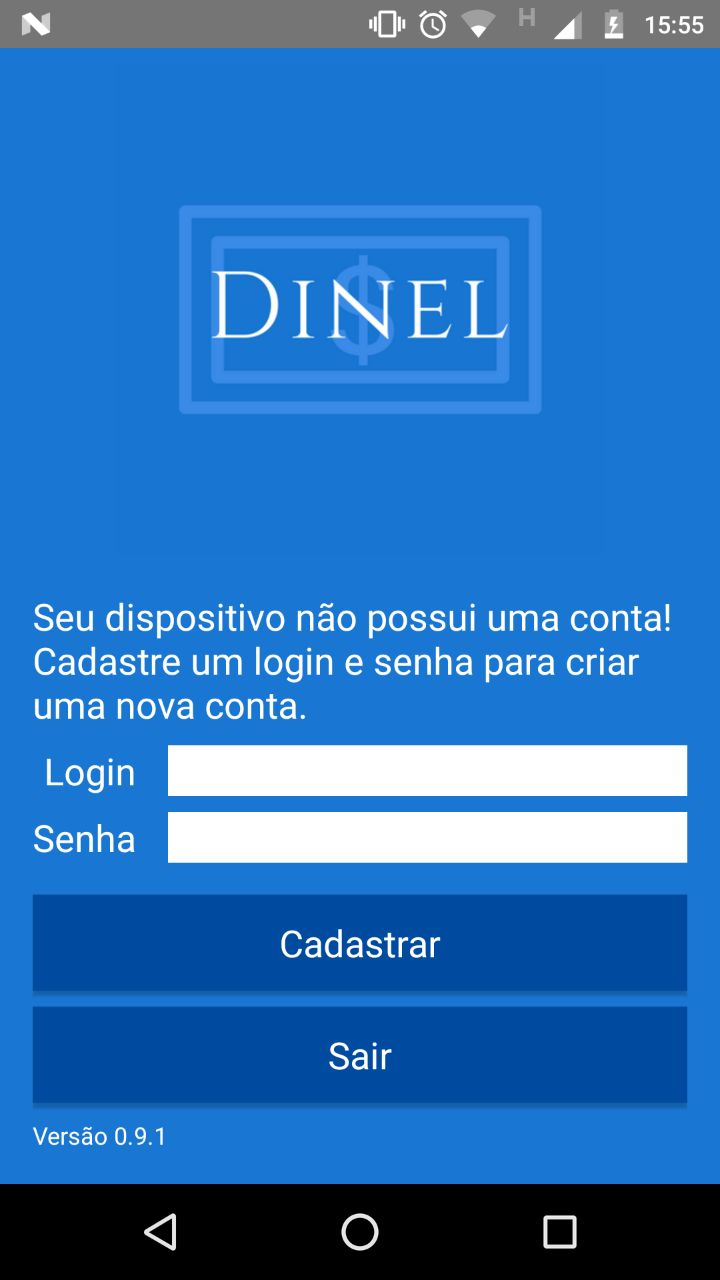
\includegraphics[scale=0.3]{cadastro} 
	\caption{Interface de cadastro de usu\'ario'}
	\label{cadastro}
\end{figure}
O componente \textit{EditText}, simplificadamente, permite que o usu\'ario insira caract\'eres na interface para serem interpretados pela aplica\c{c}\~ao. Na interface eram necess\'arios que o usu\'ario entrasse com duas \textit{strings}, uma para que ele definisse qual o nome de usu\'ario e outra para a senha. A de entrada do nome de usu\'ario foi mais direta a aplica\c{c}\~ao, a entrada de \textit{strings} \'e um componente padr\~ao que n\~ao precisou de muita configura\c{c}\~ao, a de senha era necess\'ario aplicar uma m\'ascara que ocultasse os caract\'eres a medida que eles fossem digitados, por quest\~ao de seguran\c{c}a e privacidade, o efeito desejado foi facilmente obtido apenas atribuindo o valor \textit{textPassword} na propriedade \textit{InputType} (exemplo na imagem \ref{login_pass}), essa propriedade \'e a que controla, nesse caso, se deve ser aplicado uma m\'ascara de senha, ou como ser\'a visto mais a frente, se o teclado de entrada deve exibir apenas n\'umeros ou n\'umeros e letras.

O componente \textit{Button} e o \textit{ImageView} exigiram menos customiza\c{c}\~ao para serem aplicados, o bot\~ao exigiu apenas que fossem definidos as cores de fundo e de texto que s\~ao exibidos nele, a imagem apenas que fosse indicado qual o caminho e identificador da imagem. Um ponto a ressaltar que encontrei dificuldade foi no posicionamento correto da imagem no \textit{layout}, foi preciso voltar a documenta\c{c}\~ao do \textit{Android} para entender a hierarquia de \textit{views} \cite{viewslay} e entender onde a imagem deveria ser posicionada para apresentar o comportamento esperado.

A interface de \textit{login}(imagem \ref{login}), j\'a que ela tamb\'em \'e uma das interfaces de entrada do aplicativo, como já explicado essa tela ap\'os o usu\'ario se cadastras \'e a primeira que vai ser carregada, ela n\~ao precisou que fosse implementado nenhum componente novo, os usados aqui foram os mesmo da interface de cadastro descritos acima. Uma diferen\c{c}a entre elas \'e que como a \'unica entrada de texto necess\'ario \'e a senha do usu\'ario n\~ao foram usados \textit{TextView} para indicar o que \'e para ser iserido no campo, em seu lugar foi usado a propriedade \textit{hint} que, como o nome indica, exibe uma dica para o usu\'ario do que deve ser colocado no campo, e desaparece quando o usu\'ario clica nele.
\begin{figure}[H]
	\begin{subfigure}{0.5\textwidth}
		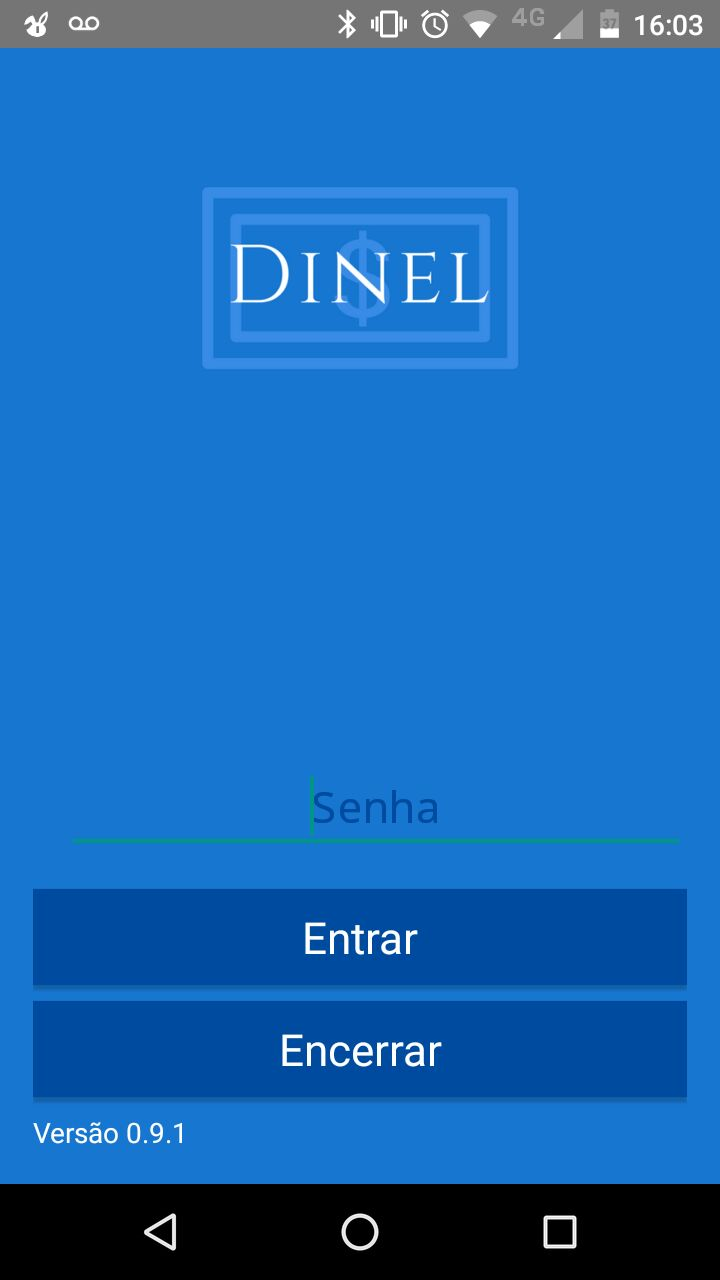
\includegraphics[scale=0.3]{login} 
		\caption{Interface de \textit{login} do aplicativo}
		\label{login}
	\end{subfigure}
	\begin{subfigure}{0.5\textwidth}
		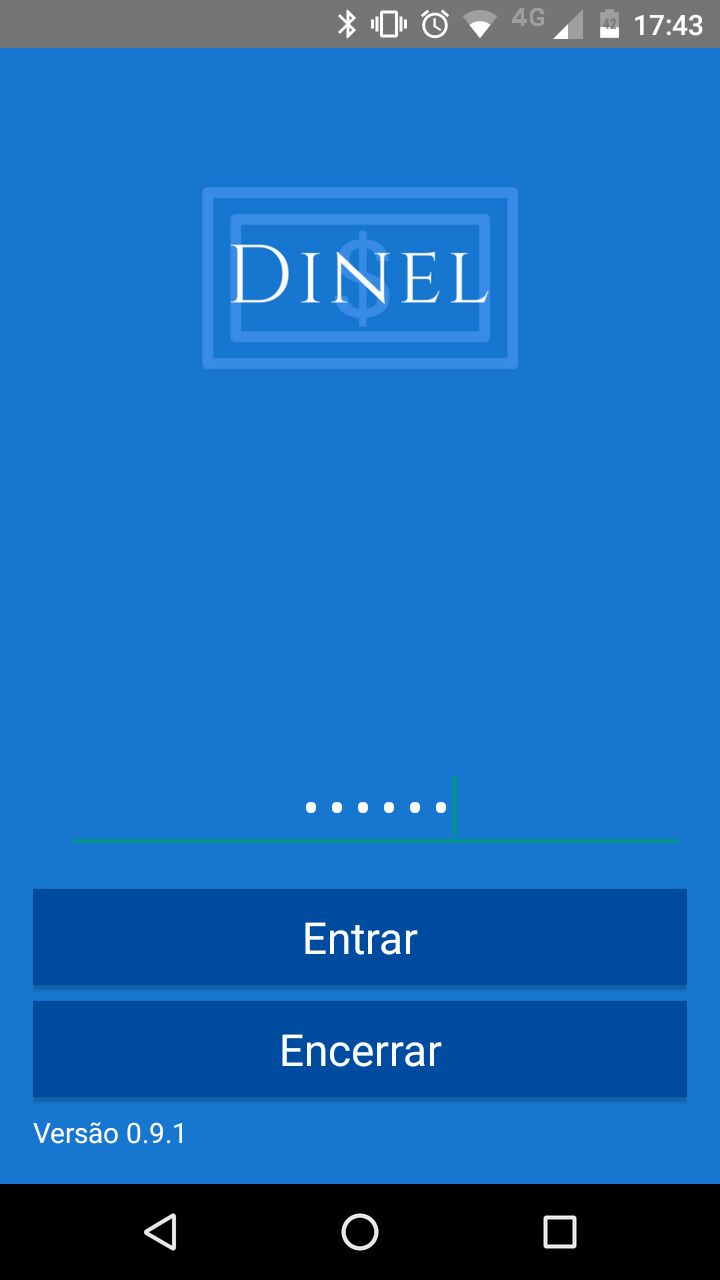
\includegraphics[scale=0.3]{login_pass}
		\caption{Campo de senha preenchido}
		\label{login_pass}
	\end{subfigure}
	\caption{Demonstra\c{c}\~ao do uso de \textit{hint} e preenchimento de campo com atributo \textit{textPassword}}
	\label{pass}
\end{figure}

A interface principal do aplicativo \'e de onde o usu\'ario pode selecionar qual a\c{c}\~ao ele deseja tomar, se ele deseja fazer um micropagamento, se quer receber, fazer uma carga de cr\'editos ou encerrar a sess\~ao, todas essas a\c{c}\~oes foram mapeadas para bot\~oes dispostos em formatos de blocos. Nessa interface foram adicionados \'icones nos bot\~oes para simbolizar cada uma das a\c{c}\~oes, como por um exemplo a imagem de um cart\~ao \ref{icon_pay} para indicar que \'e um micropagamento a ser efetuado. Nenhum componente diferente dos citados at\'e agora foi usado nesse momento. O ponto de aten\c{c}\~ao nesse tela foi tomar cuidado com o identificador que foi atribu\'ido para cada um dos bot\~oes, j\'a que no \textit{back-end} os m\'etodos que disparam cada a\c{c}\~ao buscam por esse identificador, um nome colocado errado em alguma das pontas pode ocasionar que a a\c{c}\~ao~desejada n\~ao seja disparada ou que outra seja ativada no seu lugar. Dito isso a interface pode ser vista na imagem \ref{main}.
\begin{figure}[H]
	\centering
	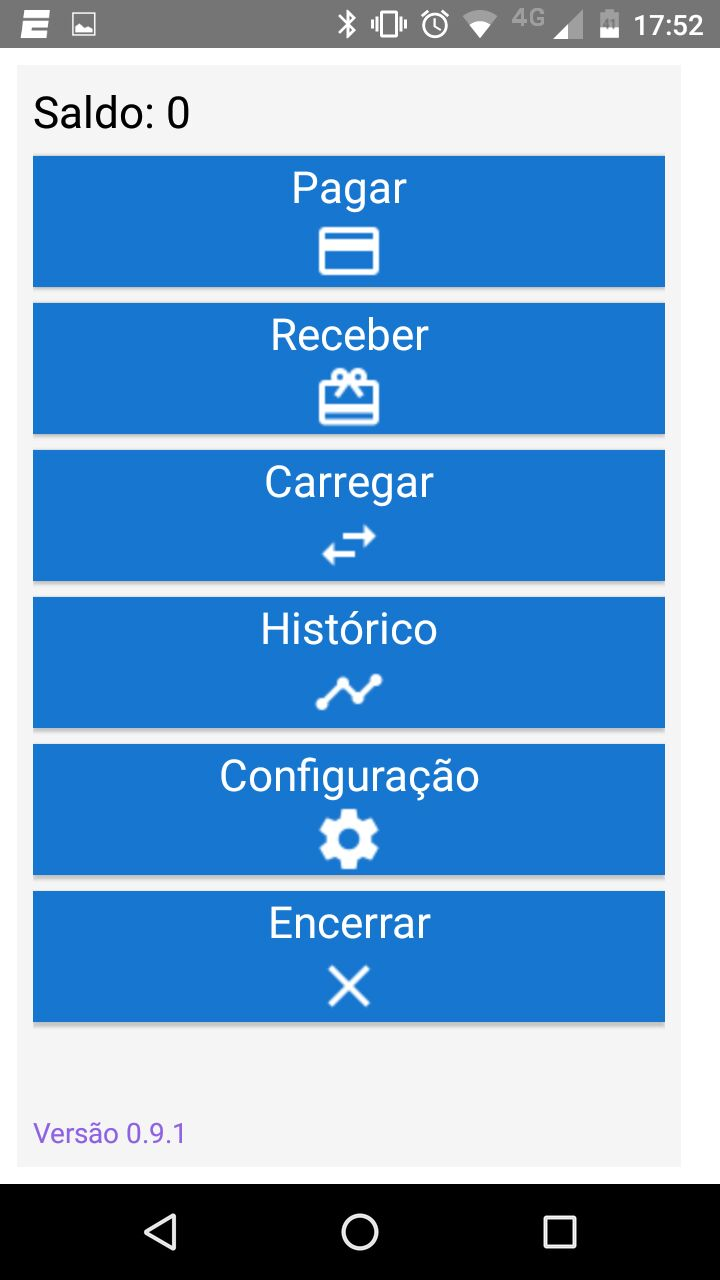
\includegraphics[scale=0.3]{main} 
	\caption{Interface principal do aplicativo}
	\label{main}
\end{figure}

A principal a\c{c}\~ao do aplicativo \'e a de efetuar um micropagamento, o fluxo de pagamento envolve dois usu\'arios e 4 interfaces no caso de sucesso, a de sele\c{c}\~ao de cedente, confirma\c{c}\~ao de transa\c{c}\~ao do lado do pagante, aguardando conex\~ao e confirma\c{c}\~ao de transa\c{c}\~ao do lado do recebente.
Iniciando pelo lado do pagante, como j\'a dito s\~ao duas interfaces, a primeira o usu\'ario efetuando o pagamento vai selecionar numa lista, obtida com base nos usu\'arios com quem ele j\'a pareou o aparelho, e confirmar ou cancelar a transa\c{c}\~ao. Na interface de sele\c{c}\~ao foi usado o componente \textit{Spinner}, ele  \'e um componente que permite selecionar um valor de uma lista de op\c{c}\~oes poss\'iveis, quando n\~ao selecionado ele assume um valor padr\~ao pr\'e-definido, quando selecionado ele exibe em uma lista todos os valores dispon\'iveis, quando um valor \'e selecionado ele fica exibido onde previamente estava o valor padr\~ao. Este comportamento pode ser observado na imagem \ref{spinner}, está exemplificado o componente selecionado (imagem \ref{spinner_on}) e como ele fica após um valor ter sido selecionado (imagem \ref{spinner_sel})
\begin{figure}[H]
	\begin{subfigure}{0.5\textwidth}
		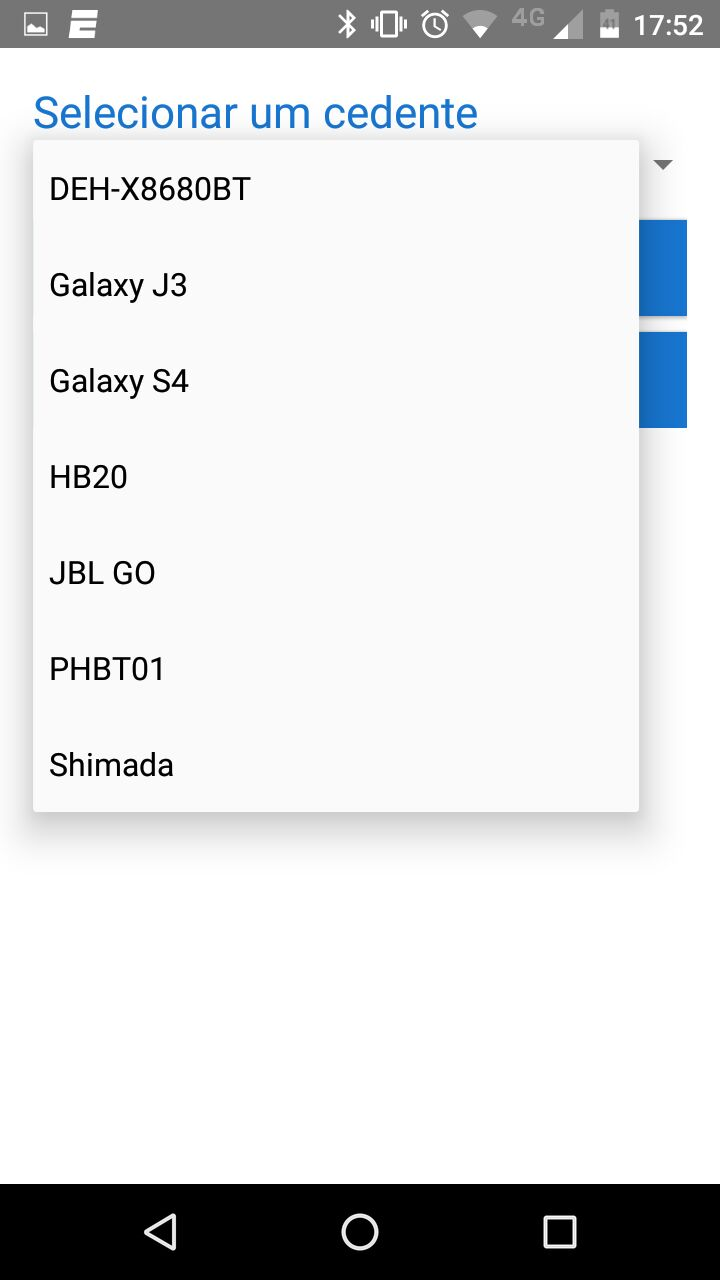
\includegraphics[scale=0.3]{spinner_on} 
		\caption{\textit{Spinner} selecionado}
		\label{spinner_on}
	\end{subfigure}
	\begin{subfigure}{0.5\textwidth}
		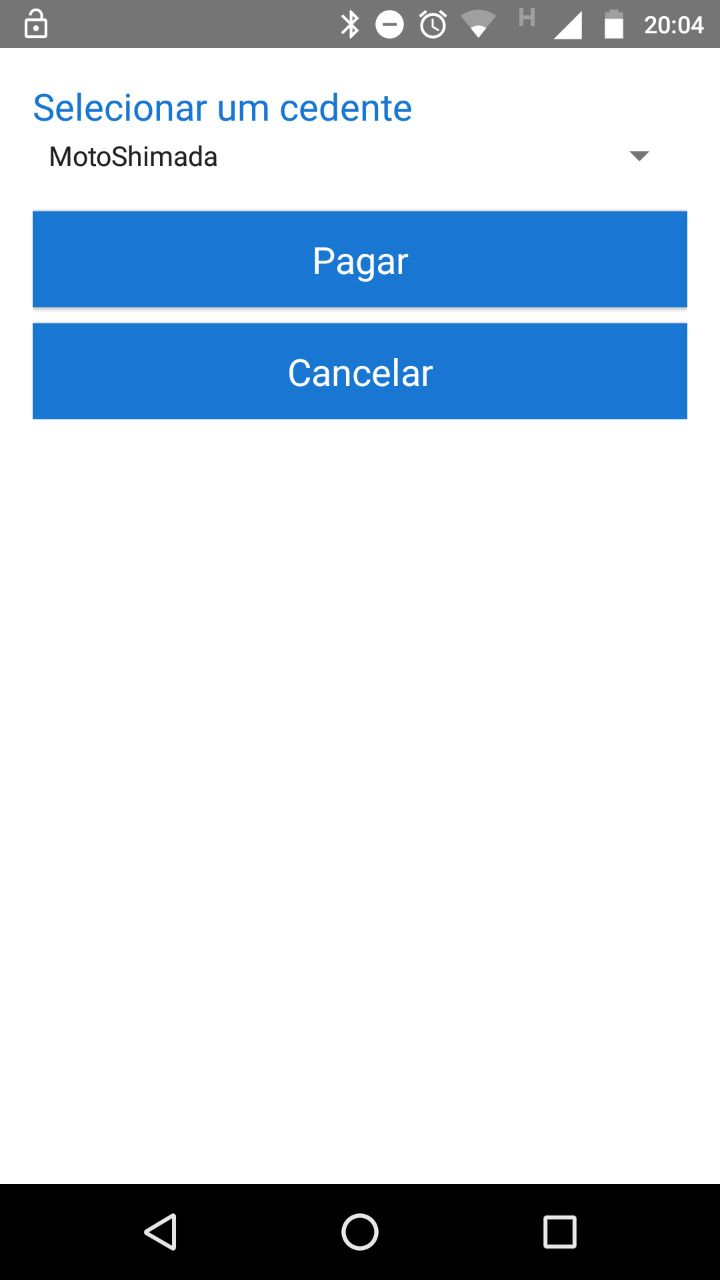
\includegraphics[scale=0.3]{spinner_selected}
		\caption{Valor selecionado no \textit{Spinner}}
		\label{spinner_sel}
	\end{subfigure}
	\caption{Demonstra\c{c}\~ao do uso do \textit{Spinner}}
	\label{spinner}
\end{figure}
Na interface \'e necess\'ario apenas adicionar o elemento \textit{\textless{Spinner}\textgreater} no c\'odigo, com suas respectivas propriedades, e na parte do controlador \'e preciso sobreescrever os m\'etodos que definem o que deve ser feito quando o usu\'ario seleciona um item e o que deve ser feito se nada for selecionado.

Do lado do recebente é exibida a interface que indica que está aguardando a conexão \textit{Bluetooth} do pagante, é exibido o logo do \textit{Bluetooth} junto com uma mensagem informando ao usuário o que o aplicativo está executando, no caso aguardando o sinal do outro \textit{smartphone}, é importante oferecer um \textit{feedback} para o usuário para ele entender que a aplicação não está travada ou que parou de funcionar. Esta interface está disponível na imagem \ref{bt}.
\begin{figure}[H]
	\centering
	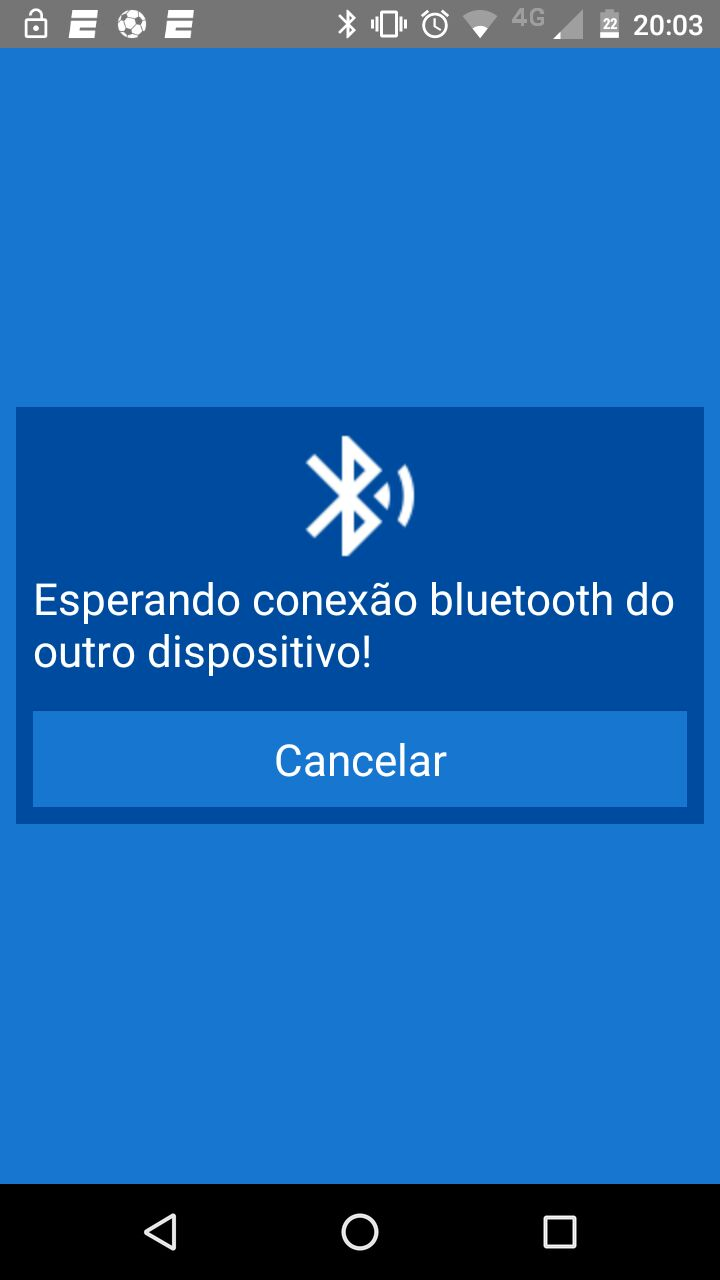
\includegraphics[scale=0.3]{wait_bt} 
	\caption{Interface do recebente aguardando contato por \textit{Bluetooth}}
	\label{bt}
\end{figure}
A interface de confirma\c{c}\~ao do pagamento que existe nos dois lados do pagamento \'e a mesma, alterando apenas a mensagem que \'e exibida para o usu\'ario, do lado do pagante \'e carregada mensagem \textbf{"Pagamento efetuado"} (imagem \ref{pay_p}), enquanto que no recebente \'e exibida a mensagem \textbf{"Recebido"} (imagem \ref{pay_r}). É renderizado tamb\'em um \'icone de "finaliza\c{c}\~ao" (\textit{done} no reposit\'orio de \'icones do \textit{Android} \cite{materialicon}), os dois componentes mais um bot\~ao para retornar ao menu inicial s\~ao exibidos dentro de um \textit{RelativeLayout} que assume o formato de uma caixa
\begin{figure}[H]
	\begin{subfigure}{0.5\textwidth}
		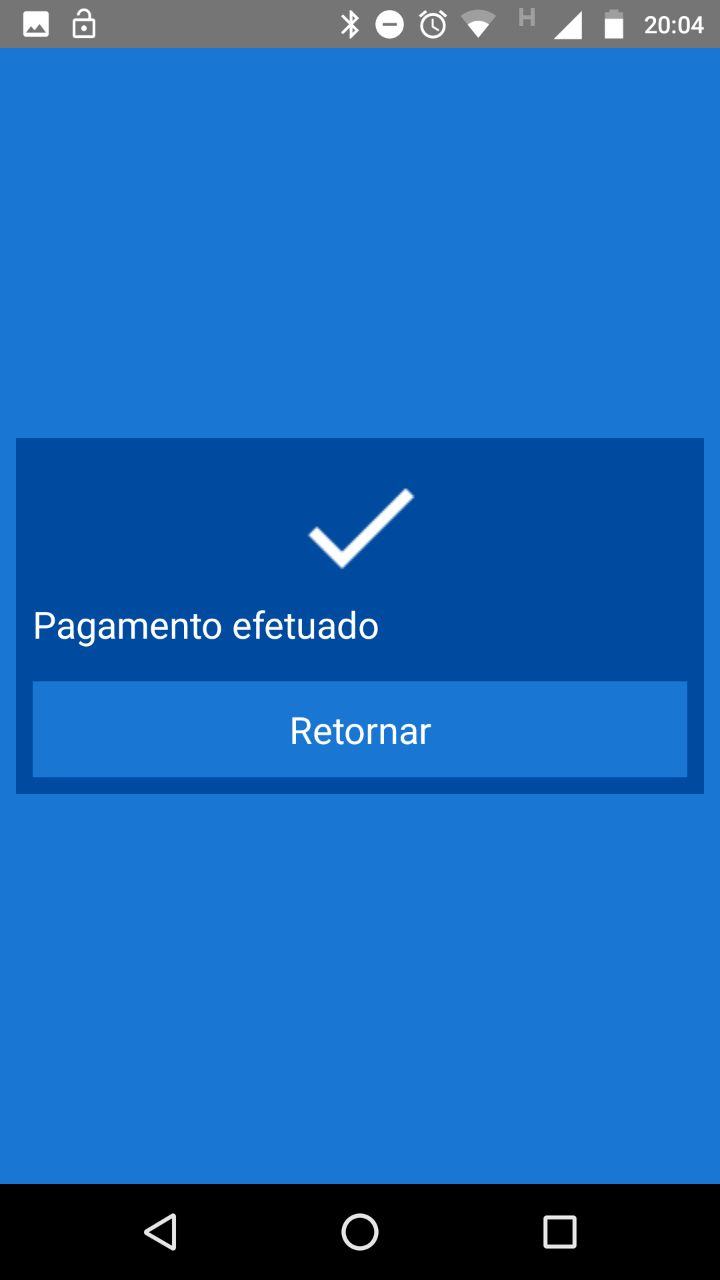
\includegraphics[scale=0.3]{pay_ok} 
		\caption{Confirma\c{c}\~ao do lado do pagante}
		\label{pay_p}
	\end{subfigure}
	\begin{subfigure}{0.5\textwidth}
		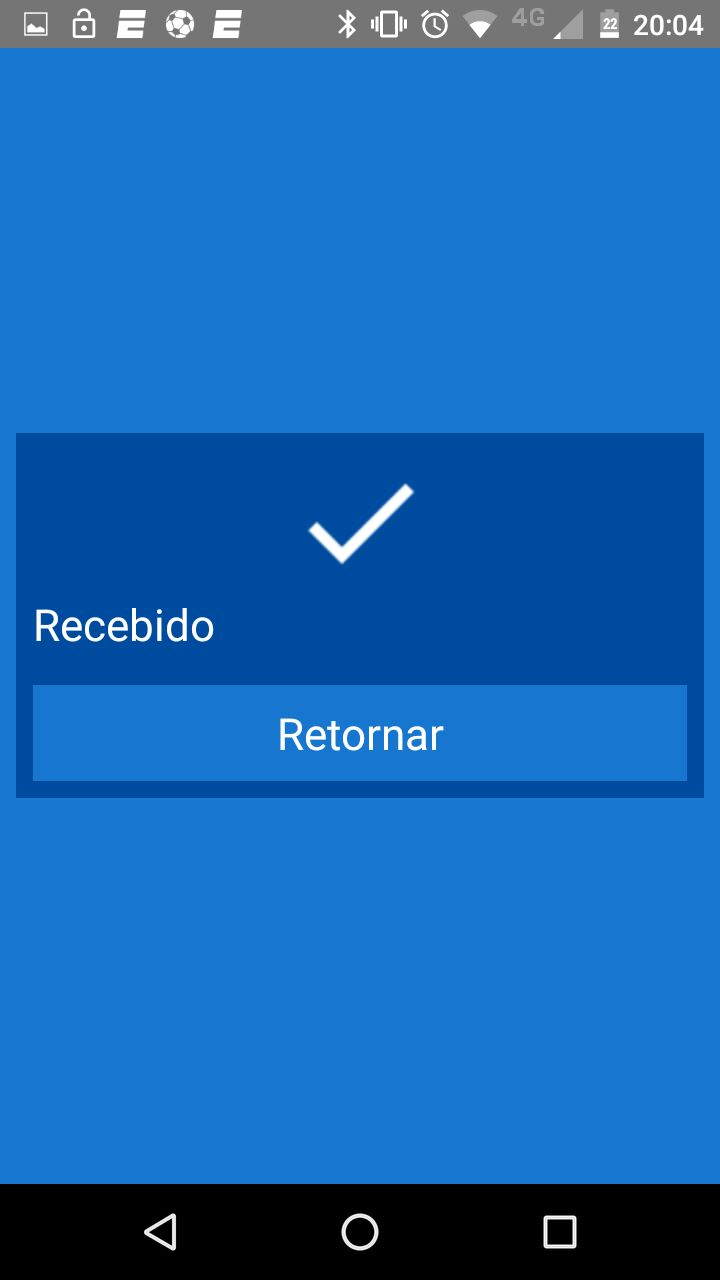
\includegraphics[scale=0.3]{pay_receive}
		\caption{Confirma\c{c}\~ao do lado do recebente}
		\label{pay_r}
	\end{subfigure}
	\caption{Interfaces de confirma\c{c}\~ao de pagamento}
	\label{pay}
\end{figure}

A outra a\c{c}\~ao desenvolvida foi a de carregamento, envolve duas interfaces (imagem \ref{charge_s}, uma principal onde s\~ao consultados os valores dispon\'iveis, e \'e poss\'ivel selecionar o quanto ser\'a carregado no aplicativo \ref{charge}, al\'em da tela de confirma\c{c}\~ao da a\c{c}\~ao. Na interface de carregamento foi usado uma propriedade diferente no campo \textit{EditText}, como \'e um campo em que ser\'a inserido um valor monet\'ario \'e esperado que sejam inseridos apenas n\'umeros no campo, para for\c{c}ar que apenas n\'umeros sejam exibidos para o usu\'ario preencher no campo foi usado o valor \textit{"number"} no atributo \textit{InputType}, esse comportamento pode ser verificado na imagem \ref{charge_numbers}. Na interface existem tamb\'em mais dois bot\~oes que n\~ao exigiram nenhuma configura\c{c}\~ao especial para atingirem o efeito desejado.
\begin{figure}[H]
	\begin{subfigure}{0.5\textwidth}
		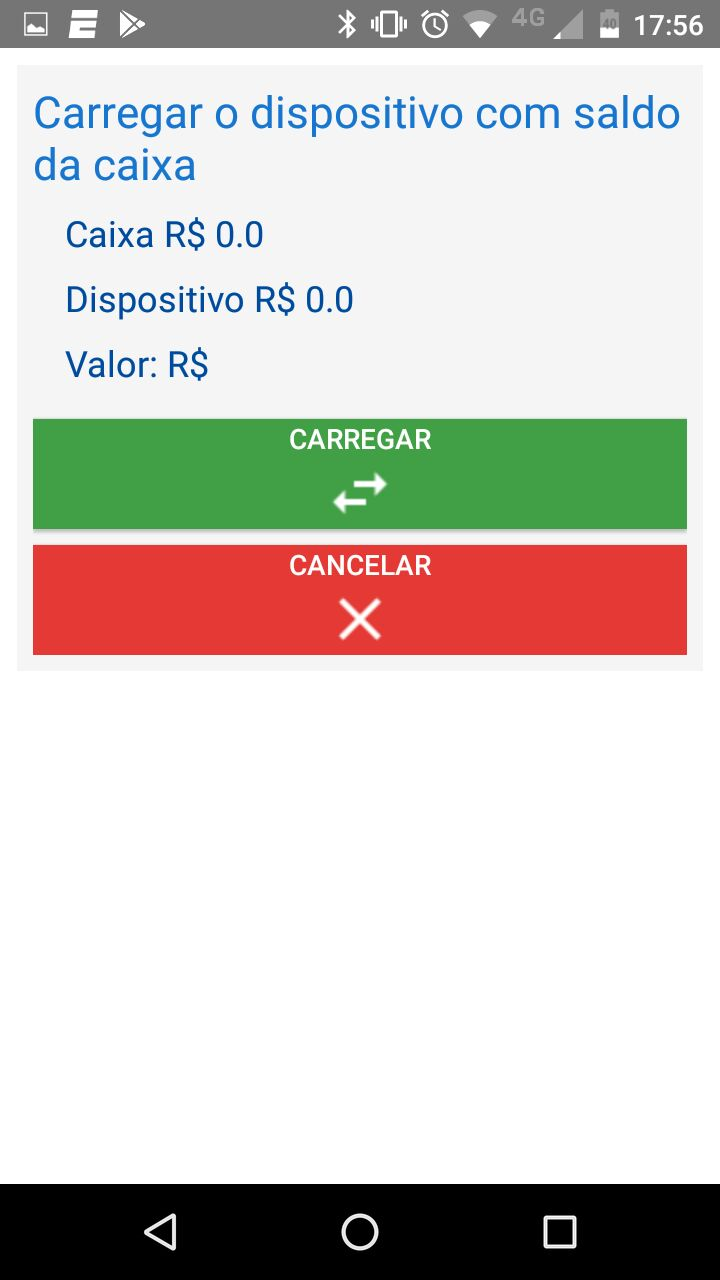
\includegraphics[scale=0.3]{charge_on} 
		\caption{Interface de carregamento}
		\label{charge}
	\end{subfigure}
	\begin{subfigure}{0.5\textwidth}
		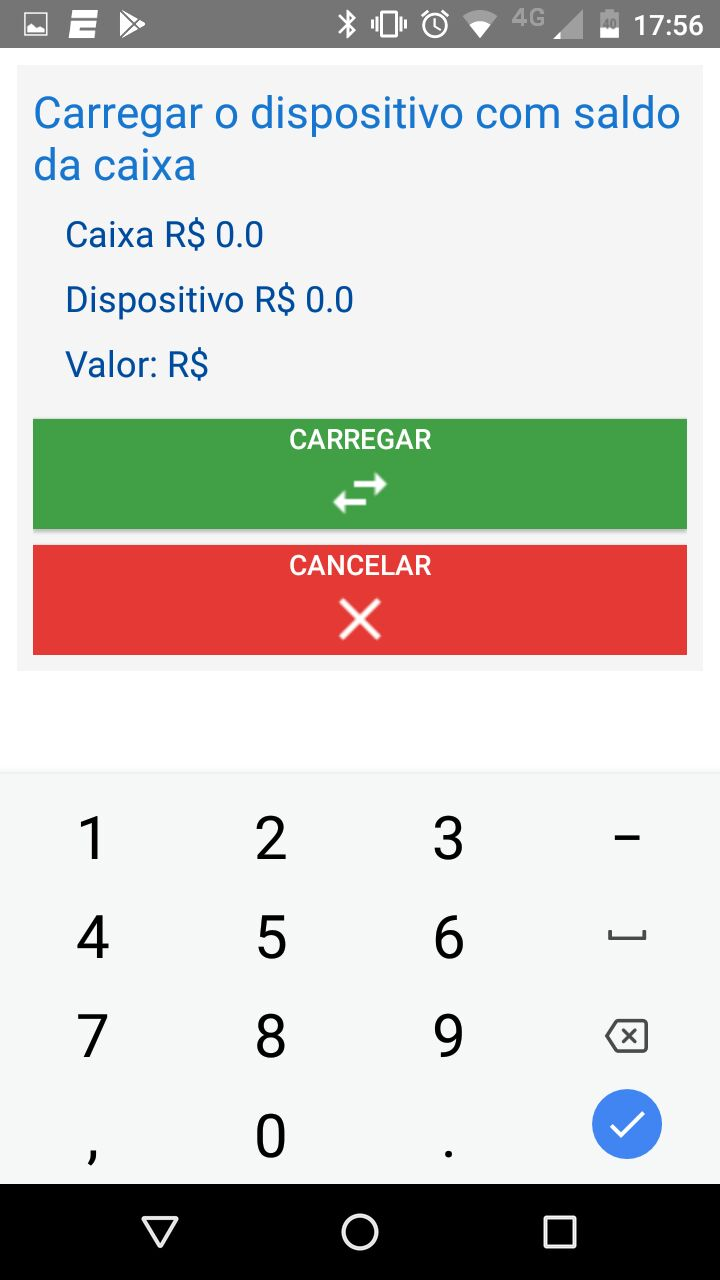
\includegraphics[scale=0.3]{charge}
		\caption{Teclado apenas com op\c{c}\~oes de n\'umeros}
		\label{charge_numbers}
	\end{subfigure}
	\caption{Interfaces de carregamento de valores}
	\label{charge_s}
\end{figure}

Infelizmente at\'e o encerramento do trabalho a plataforma de servi\c{c}os ainda estava apresentando erro no momento de confirma\c{c}\~ao do carregamento, por esse motivo n\~ao foi poss\'ivel em tempo de execu\c{c}\~ao obter as imagens de confirma\c{c}\~ao da aplica\c{c}\~ao.

Isto porque as mensagens de confirma\c{c}\~ao e erro,etc, s\~ao uma cole\c{c}\~ao de 3 interfaces que s\~ao usadas dinamicamente ao longo do aplicativo, mudando apenas o texto que \'e carregado dependendo de cada contexto que essas interfaces s\~ao carregadas para serem exibidas, um exemplo do uso delas pode ser visto nas imagens \ref{pay_p}, \ref{pay_r} e \ref{bt}. As mensagens de erro n\~ao foram descritas em detalhes por conta da implementa\c{c}\~ao que foi feita, mas como exemplo, temos a mensagem de erro exibida caso o usu\'ario entre com a senha errada, \'e carregada no \textit{template} um \'icone simbolizando que \'e preciso aten\c{c}\~ao, e a mensagem explicando o motivo da aten\c{c}\~ao, no caso a senha que foi colocada de forma incorreta, este exemplo pode ser visto na imagem \ref{error}.
\begin{figure}[H]
	\centering
	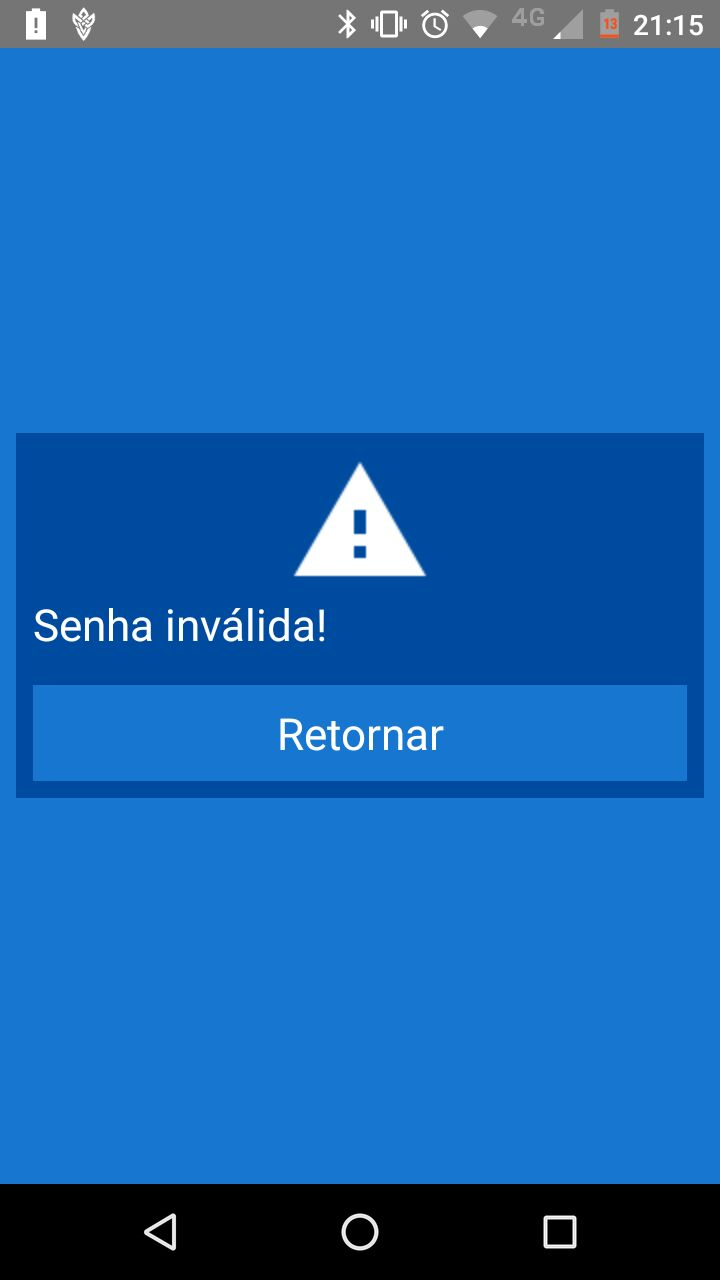
\includegraphics[scale=0.3]{error} 
	\caption{Alerta de erro}
	\label{error}
\end{figure}

Devido ao grande n\'umero de \textit{strings} usadas no aplicativo, foi usado um arquivo \textit{XML} para armazenar todas as usadas no aplicativo. As vantagens dessa abordagem, ao contr\'ario de escrever manualmente todas elas diretamente, \'e a flexibilidade e a reusabilidade.

Flexibilidade pois tendo o arquivo como base \'e poss\'ivel traduzir ele para outros idiomas, como o id das \textit{strings} permanece o mesmo, as mesmas j\'a est\~ao referenciadas no c\'odigo e v\~ao exibir o valor definido. Isto \'e \'util para se localizar o aplicativo para outros pa\'ises que usam uma linguagem diferente da que se foi desenvolvido o aplicativo inicialmente.

Reusabilidade porque elas s\~ao apenas referenciadas no c\'odigo, qualquer mudan\c{c}a que for feita em um dos valores \'e replicada por todo o aplicativo poupando o trabalho de precisar reescrever todas as ocorrências e correr o risco de esquecer alguma, al\'em da possibilidade de usar uma mesma palavra em diversos elementos do aplicativo sem a necessidade de escrever o mesmo repetidas vezes.
% end new block% end new block% end new block
% end new block% end new block% end new block
% end new block% end new block% end new block
\subsection{Intergra\c{c}\~ao com a plataforma de servi\c{c}os} \label{dev}

Finalizada a etapa de desenvolvimento das interfaces, dei in\'icio ao segundo objetivo do trabalho que consistia em integrar as interfaces do aplicativo de micropagamento para operar com uma base de servi\c{c}os funcional. O primeiro passo foi a familiariza\c{c}\~ao com a plataforma, entender o fluxo de execu\c{c}\~ao, os triggers, os listeners, estudar literalmente a plataforma inteira, nessa parte contei com a colabora\c{c}\~ao do Henrique Leme, desenvolvedor da plataforma, com o aux\'ilio dele essa parte foi facilitada permitindo que a assimila\c{c}\~ao do conte\'udo fosse mais flu\'ida.

Como as interfaces foram desenhadas j\'a com o conhecimento pr\'evio da base de servi\c{c}os, n\~ao foram encontradas muitas dificuldades para fazer essa integra\c{c}\~ao, j\'a que as interfaces foram feitas com os campos que cada a\c{c}\~ao precisava para ser executada, o risco maior de ter que refazer todas elas foi mitigado.

O ponto principal desse momento do trabalho foi o cuidado de nomear corretamente cada interface desenhada e seus componentes e mapear eles no controlador da aplica\c{c}\~ao. J\'a que como descrito anteriormente isso pode acarretar uma s\'erie de problemas como a\c{c}\~oes indesejadas sendo disparadas no lugar de outras, campos que n\~ao tem seus valores capturados de forma correta, etc.

A estrutura do \textit{back-end} do aplicativo se comporta como ilustrado na imagem \ref{estrut}, a estrutura para funcionar envolvem dois \textit{smartphones} (identificados como "Dipositivos"), um servidor para efetuar e gerenciar as transa\c{c}\~oes dos micropagamentos e um servidor de dados colhendo e armazenando as informa\c{c}\~oes das transa\c{c}\~oes e usu\'arios.
\begin{figure}[H]
	\centering
	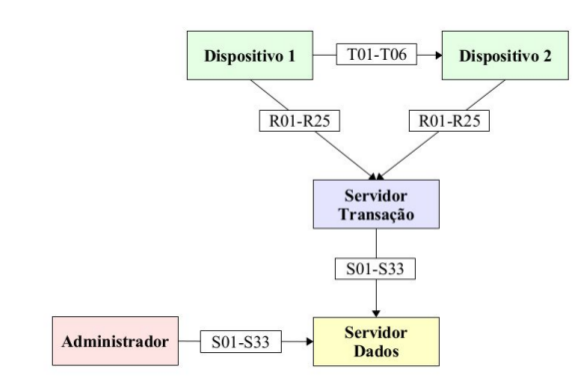
\includegraphics[scale=0.5]{estrutura} 
	\caption{Estrutura do \textit{back-end}}
	\label{estrut}
\end{figure}
Os dispositivos conversam entre si usando um conjunto de seis opera\c{c}\~oes:
\begin{itemize}
	\item T1 - Um dispositivo A se torna dispon\'ivel para receber um micropagamento
	\item T2 - Um dispositivo B entra em contato com A para informar que quer fazer o micropagamento
	\item T3 - O dispositivo A aceita o dispostivo o B
	\item T4 - O dispositivo B realiza a transa\c{c}\~ao
	\item T5 - O dispostivo A confirma a transa\c{c}\~ao
	\item T6 - Existe uma opera\c{c}\~ao de cancelamento que pode ser executada por qualquer uma das duas partes
\end{itemize}
Essa opera\c{c}\~oes podem ser vistas no diagrama da imagem \ref{transactions}, onde A \'e o cedente e B \'e o sacado.
\begin{figure}[H]
	\centering
	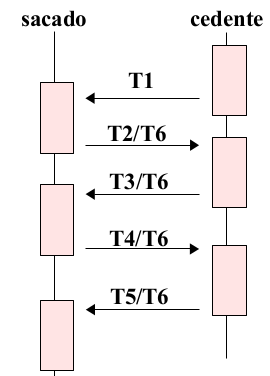
\includegraphics[scale=0.5]{transactions} 
	\caption{Opera\c{c}\~oes entre dispositivos}
	\label{transactions}
\end{figure}

\section{Considera\c{c}\~oes Finais}
No in\'icio do projeto foram definidos dois objetivos para este trabalho, aprender o desenvolvimento para \textit{Android} e aplicar o conhecimento adquirido para produzir as interfaces de um aplicativo. Sendo o primeiro pr\'e-requisito obrigat\'orio para a execu\c{c}\~ao do segundo, \'e mais prudente discorrer sobre ele de in\'icio.

O desenvolvimento para \textit{Android} conta com uma boa base de conhecimento e materiais no pr\'oprio site tanto de t\'opicos b\'asicos, como por exemplo um guia de configura\c{c}\~ao do ambiente, at\'e mais avan\c{c}ados, como a documenta\c{c}\~ao de cada componente da plataforma, que pode ser considerado suficiente para qualquer um que tenha interesse em aprender a desenvolver aplicativos para \textit{Android} consiga fazer o mesmo. É bem verdade que em alguns assuntos a documenta\c{c}\~ao \'e um pouco confusa ou peca pela falta de exemplos mais concretos de implementa\c{c}\~ao, mas, como dito na se\c{c}\~ao \ref{revisao}, f\'oruns e sites na internet existem em grandes quantidades com outras pessoas com d\'uvidas similares ou aproximadamente iguais, e a maoria com solu\c{c}\~oes para tais empecilhos. Um problema recorrente nisso \'e talvez a falta de uma solu\c{c}\~ao \'unica, para um mesmo problema podem existir n solu\c{c}\~oes diferentes, o que exige muita an\'alise e testes para descobrir quais, ou qual, \'e a mais adequada para o problema encontrado.

Isso era comum de se encontrar tanto para problemas de interfaces, como por exemplo como fazer uma imagem caber dentro de um bot\~ao, como para problemas de \textit{back-end}, como por exemplo qual a melhor abordagem para implementar \textit{Fragments} em elementos do \textit{layout}.

Apesar disso considero que a plataforma apresenta uma dificuldade m\'edia de aprendizado, alguns elementos s\~ao de f\'acil assimila\c{c}\~ao ao passo que alguns exigem um pouco mais de estudo e pesquisa para se entender o que precisa ser feito para atingir o resultado esperado. As interfaces s\~ao mais f\'aceis de compreender como se desenvolver do que como prograrmar os controles que gerenciam o funcionamento da aplica\c{c}\~ao.

Considero que \'e poss\'ivel sim aprender sozinho o suficiente para criar um aplicativo simples usando as informa\c{c}\~oes que se encontra nas documenta\c{c}oes oficiais e nas literaturas sobre o assunto, mas para projetos de larga escala acredito ser dif\'icil de conseguir o resultado desejado apenas com esses recursos.

Quanto ao segundo objetivo, mantenho o que foi dissertado na sub-se\c{c}\~ao \ref{dev} em rela\c{c}\~ao ao desenvolvimento das mesmas, uma das premissas era que as interfaces do aplicativo fossem de f\'acil usablidade, com isso em foco, considerei mais prudente n\~ao precisar fazer nada que fosse apenas visualmente mais atraente mas de d\'ificil asssimi\c{c}\~ao e foquei em pensar na solu\c{c}\~ao que fosse de mais f\'acil compreens\~ao qual a\c{c}\~ao deveria ser tomada em cada umas das interfaces. É claro que sem a primeira parte do aprendizado esta etapa teria possu\'ido uma dificuldade exrememamente maior de ser realizada, j\'a que ao mesmo tempo seria necess\'ario entender o funcionamento e desenvolver os componentes nas interfaces.

Uma futura possibilidade que poderia ser considerada como uma extens\~ao desse trabalho seria tentar adaptar o aplicativo usando a linguagem \textit{Kotlin}. Recentemente os respons\'aveis pelo \textit{Android} anunciaram que a plataforma passaria a oferecer suporte para a linguagem \cite{kotlin:and_adopt}. O site da \textit{Wired} publicou um artigo em que diz que a linguagem \'e a nova tendência no Vale do Sil\'icio e que passaremos a ver cada vez mais aplicativos desenvolvidos nela \cite{kotlin:wired}.

Para este trabalho em espec\'ifico o \textit{Kotlin} entrou mais como uma curiosidade, j\'a que o foco dele era desenvolvimento em \textit{Android} puro, por\'em foi algo que despertou grande curiosidade em explorar essa nova linguagem e medir a diferen\c{c}a do tempo de aprendizagem e implementa\c{c}\~ao de um aplicativo usando cada uma das linguagens.
%Final do doc
\newpage
\section*{Refer\^encias Bibliogr\'aficas}
\addcontentsline{toc}{section}{Refer\^encias Bibliogr\'aficas}
\renewcommand\refname{}
\bibliography{helper}
\bibliographystyle{unsrt}
\end{document}